
\begin{frame}{slogans \& scope}

slogans: I will
  \begin{itemize}
  \item \alert{focus on approximating ice flow}
  \item \alert{provide numerical codes that actually work}
  \item \alert{always care about the continuum model}
  \end{itemize}
\medskip

scope: I will cover these
  \begin{itemize}
  \item models

    \begin{itemize}
    \item[$\circ$] shallow ice approximation (SIA) in 2D
    \item[$\circ$] shallow shelf approximation (SSA) in 1D
    \item[$\circ$] mass continuity \& surface kinematical equations
    \end{itemize}

  \item numerical ideas

    \begin{itemize}
    \item[$\circ$] finite difference schemes
    \item[$\circ$] solving algebraic systems from stress balances
    \item[$\circ$] verification
    \end{itemize}
  \end{itemize}
\end{frame}


\begin{comment}
\begin{frame}{outside of scope}

\large\emph{not} \normalsize covered here:\normalsize
\medskip

  \begin{itemize}
  \item Stokes and ``higher order'' flow equations
  \item thermomechanical coupling or polythermal ice
  \item subglacial hydrology/processes
  \item mass balance and snow/firn processes
  \item constitutive relations other than Glen isotropic
  \item grounding lines, calving fronts, ocean interaction
  \item paleo-climate and ``spin-up''
  \item earth deformation under ice sheet load
  \item other numerics: FEM, spectral, multigrid, parallel, \dots
  \item etc.
  \end{itemize}

\end{frame}
\end{comment}

\begin{frame}{notation} 

\begin{center}
  \includegraphics[width=0.9\textwidth]{flowline}

\tiny \emph{figure modified from} Schoof (2007)
\end{center}

\scriptsize
  \begin{itemize}
  \item coordinates $t,x,y,z$  (with $z$ vertical, positive upward)
  \item subscripts for partial derivatives $u_x = \partial u/\partial x$
  \item $H=$ ice thickness
  \item $h=$ ice surface elevation
  \item $b=$ bedrock surface elevation
  \item $T=$ temperature
  \item $\mathbf{u}=(u,v,w)=$ ice velocity
  \item $\rho=$ density of ice
  \item $\rho_w=$ density of ocean water
  \item $g=$ acceleration of gravity
  \item $n$ Glen flow law exponent (usually $=3$)
  \item $A=A(T)=$ ice softness in Glen law ($\mathbf{D}_{ij} = A(T) \tau^{n-1} \tau_{ij}$)
  \item \alert{please ask about notation!}
  \end{itemize}

\end{frame}


\begin{frame}{Matlab/Octave codes}

\begin{itemize}
\item lectures and notes are based on 18 Matlab/Octave codes
\item several will appear in these lectures, but not all
\item each is $\sim$ 1/2 page
\item please give them a try!

  \begin{itemize}
  \item[$\circ$] \texttt{.zip} and \texttt{.tar.gz} forms available from USB drive
  \item[$\circ$] and online:

  \bigskip\bigskip\small
  \centerline{\fbox{\url{https://github.com/bueler/mccarthy}}}
  
  \end{itemize}
\end{itemize}
\end{frame}


\section[introduction]{introduction: a view from outside glaciology}

\begin{frame}{ice in glaciers is a \emph{fluid}}

\begin{itemize}
\item what's a fluid?
\item is it just a collection of particles?

\medskip
\item<2> its a mathematical abstraction
\item<2> \dots with equations relating these fields:
  \begin{itemize}
  \item[$\circ$] a scalar \emph{density}\quad $\rho(t,x,y,z)$
  \item[$\circ$] a scalar \emph{pressure}\quad $p(t,x,y,z)$
  \item[$\circ$] a vector \emph{velocity}\quad $\mathbf{u}(t,x,y,z)$
  \end{itemize}
\end{itemize}

\vspace{-2mm}
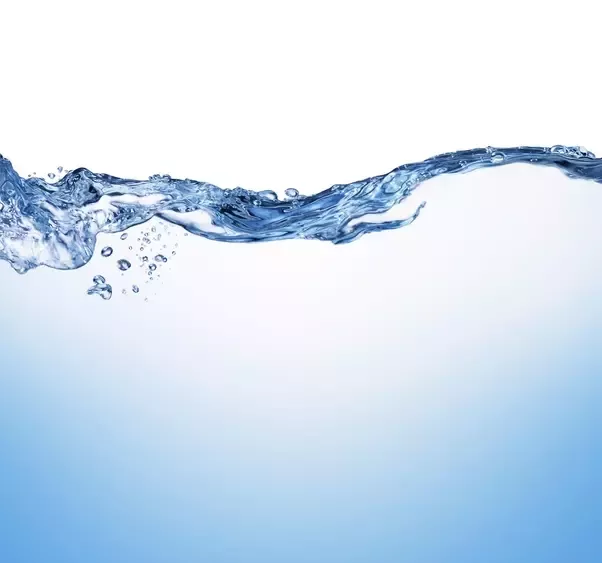
\includegraphics[width=0.4\textwidth]{liquid} \hfill \uncover<2>{
\includegraphics[width=0.35\textwidth]{lighterfluidalpha}}
\end{frame}


\begin{frame}{ice in glaciers is an atypical fluid}

\begin{itemize}
\item if the ice were
  \begin{itemize}
  \item[$\circ$] faster-moving than it actually is, and
  \item[$\circ$] linearly-viscous like liquid water
  \end{itemize}
  
  then it would be a ``typical'' fluid

\bigskip
\item for typical fluids one uses the Navier-Stokes equations:
\begin{align*}
\nabla \cdot \mathbf{u} &= 0 &&\text{\emph{incompressibility}} \\
\rho \left(\mathbf{u}_t + \mathbf{u}\cdot\nabla \mathbf{u}\right) &= -\nabla p + \nabla \cdot \tau_{ij} + \rho \mathbf{g} &&\text{\emph{stress balance}} \\
2 \nu \mathbf{D}_{ij} &= \tau_{ij} &&\text{\emph{flow law}}
\end{align*}

\medskip
    \begin{itemize}
    \item[$\circ$] stress balance equation is ``$m a = F$''
    \item[$\circ$] unclaimed \$1 million prize for showing this is a good model
    \end{itemize}
\end{itemize}
\end{frame}


\begin{frame}{glaciology as computational fluid dynamics}

\begin{itemize}
\item \alert{yes}, numerical ice sheet flow modelling is ``computational fluid dynamics''
  \begin{itemize}
  \item[$\circ$] it's large-scale like atmosphere and ocean
  \item[$\circ$] \dots\, but it is a weird one
  \end{itemize}
\item consider what makes atmosphere/ocean flow exciting:
  \begin{itemize}
  \item[$\circ$] turbulence
  \item[$\circ$] convection
  \item[$\circ$] coriolis force
  \item[$\circ$] density stratification
  \end{itemize}
\item none of the above list is relevant to ice flow
\item what could be interesting about the flow of slow, cold, stiff, laminar, inert old ice?
  \begin{itemize}
  \item[$\circ$] it's \emph{ice dynamics!}
  \end{itemize}
\end{itemize}
\end{frame}


\begin{frame}{ice is a slow, shear-thinning fluid}

\begin{itemize}
\item ice fluid is \emph{slow} and \emph{non-Newtonian}
    \begin{itemize}
    \item[$\circ$] ``slow'' is a technical term:
      $$\rho \left(\mathbf{u}_t + \mathbf{u}\cdot\nabla \mathbf{u}\right) \approx 0 \qquad \iff \qquad \begin{pmatrix} \text{forces of inertia} \\ \text{are neglected} \end{pmatrix}$$
    \item[$\circ$] ice is non-Newtonian in a ``shear-thinning'' way
        \begin{itemize}
        \item higher strain rates means lower viscosity
        \item viscosity $\nu$ is not constant
        \end{itemize}
    \end{itemize}

\bigskip
\item thus the standard model is Glen-law Stokes:
\begin{align*}
\nabla \cdot \mathbf{u} &= 0 &&\text{\emph{incompressibility}} \\
0 &= - \nabla p + \nabla \cdot \tau_{ij} + \rho\, \mathbf{g} &&\text{\emph{stress balance}} \\
\mathbf{D}_{ij} &= A \tau^{n-1} \tau_{ij} &&\text{\emph{flow law}}
\end{align*}

\end{itemize}
\end{frame}


\begin{frame}{``slow'' means no memory of velocity/momentum}

\begin{itemize}
\item note \emph{no time derivatives} in Stokes model:
\small
\begin{align*}
\nabla \cdot \mathbf{u} &= 0 \\
0 &= - \nabla p + \nabla \cdot \tau_{ij} + \rho\, \mathbf{g} \\
\mathbf{D}_{ij} &= A \tau^{n-1} \tau_{ij}
\end{align*}
\normalsize
\item thus a time-stepping ice sheet code recomputes the full velocity field at every time step
  \begin{itemize}
  \item[$\circ$] it does not require velocity from the previous time step\footnote{you don't need \dots to know which way the wind blows}
  \end{itemize}
\item velocity is a ``diagnostic'' output not needed for starting or restarting the model
\end{itemize}
\end{frame}


\begin{frame}{plane flow Stokes}

\begin{itemize}
\item suppose we work in a $x,z$ plane, such as the centerline of a glacier, or a cross-flow plane
\item now the $n=3$ Stokes equations say
\begin{empheq}[]{align}
u_x + w_z &= 0 &&\text{\emph{incompressibility}}\notag \\
p_x &= \tau_{11,x} + \tau_{13,z} &&\text{\emph{stress balance} ($x$)} \notag \\
p_z &= \tau_{13,x} - \tau_{11,z} - \rho g &&\text{\emph{stress balance} ($z$)} \notag \\
u_x &= A \tau^2 \tau_{11} &&\text{\emph{flow law (diagonal)}}\notag \\
u_z + w _x &= 2 A \tau^2 \tau_{13} &&\text{\emph{flow law (off-diagonal)}} \notag
\end{empheq}

\vspace{-2mm}
    \begin{itemize}
    \item[$\circ$] \emph{notation}: subscripts $x,z$ denote partial derivatives, $\tau_{13}$ is the ``vertical'' shear stress, $\tau_{11}$ and $\tau_{33}=-\tau_{11}$ are (deviatoric) longitudinal stresses
    \end{itemize}
\item we have five equations in five unknowns ($u,w,p,\tau_{11},\tau_{13}$)
\item this is complicated enough \dots what about in a simplified situation?
\end{itemize}
\end{frame}


\begin{frame}{slab-on-a-slope}

\hfill \includegraphics[width=0.4\textwidth]{slab}

\vspace{-30mm}
\begin{itemize}
\item suppose constant thickness
\item tilt bedrock by angle $\alpha$
\item rotate the coordinates
\item get these new expressions:
\begin{align*}
\mathbf{g} &= g \sin\alpha\, \hat x - g \cos \alpha \,\hat z \phantom{dslfkj sdkfjlskdjf  sdlfj}\\
p_x &= \tau_{11,x} + \tau_{13,z} + \rho g \sin\alpha \\
p_z &= \tau_{13,x} - \tau_{11,z} - \rho g \cos\alpha
\end{align*}
\item for this \alert{slab-on-a-slope} there is \emph{no variation in} $x$: $\partial/\partial x = 0$
\item the equations simplify:
\small
\begin{empheq}[box=\fbox]{align}
w_z &= 0 &   0 &= \tau_{11} \notag \\
\tau_{13,z} &= - \rho g \sin\alpha &   u_z &= 2 A \tau^2 \tau_{13} \notag \\
p_z &= - \rho g \cos\alpha \notag
\end{empheq}
\end{itemize}

\end{frame}


\begin{frame}{slab-on-a-slope 2}

\begin{itemize}
\item add boundary conditions:
	$$w(\text{base})=0, \qquad p(\text{surface})=0, \qquad u(\text{base})=u_0$$
\item by integrating vertically, get:
\begin{align*}
w &= 0 \phantom{asdfklj asldkfjalk asdfkj sdlfkj sldafkj adlfjl sdfakj }\\
p &= \rho g \cos\alpha (H-z) \\
\tau_{13} &= \rho g \sin\alpha (H-z)
\end{align*}

\vspace{-25mm}
\hfill \includegraphics[width=0.4\textwidth]{slabshear}

\vspace{-7mm}
\item $\tau_{13}$ is linear in depth

\medskip
\item from $u_z = 2 A \tau^2 \tau_{13}$ get \alert{velocity formula}
\vspace{-0.05in}
\begin{align*}
u(z) &= u_0 + 2 A (\rho g \sin\alpha)^3 \int_0^z (H-z')^3\,dz' \\
     &= u_0 + \frac{1}{2} A (\rho g \sin\alpha)^3  \left(H^4 - (H-z)^4\right)
\end{align*}
\end{itemize}
\end{frame}


\begin{frame}{slab-on-a-slope 3}

\begin{columns}
\begin{column}{0.6\textwidth}
\begin{itemize}
\item do we believe these equations?
\item velocity formula on last slide gives figure below
\item compare to observations at right
\end{itemize}
\begin{center}
% NOT preserving aspect ratio
\includegraphics[width=0.6\textwidth,height=0.5\textheight]{slabvel}
\end{center}
\end{column}

\begin{column}{0.4\textwidth}
\includegraphics[width=1.0\textwidth]{athabasca-deform}

\medskip
\scriptsize
Velocity profile of the Athabasca Glacier, Canada, derived from inclinometry (Savage and Paterson, 1963)
\end{column}
\end{columns}
\end{frame}


\begin{frame}{mass conservation}

\small
\begin{itemize}
\item[Q:] having computed the velocity $u=u(t,x,z)$ \dots so what?
\item[A:] velocity partly determines the new ice shape through \alert{mass conservation}
\item suppose our ice has variable thickness $H(t,x)$
\item define the vertical average of velocity:
	$$\bar U(t,x) = \frac{1}{H}\int_0^{H} u(t,x,z)\,dz \phantom{sdlj asdlbj asldbfj asdlfj}$$

\vspace{-20mm}
\hfill \includegraphics[width=0.3\textwidth]{slabmasscontfig}
\item with climatic mass balance $M(x)$, consider change of area in the figure:
	$$\frac{dA}{dt} = \int_{x_1}^{x_2} M(x)\,dx + \bar U_1 H_1 - \bar U_2 H_2$$

    \vspace{-2mm}
    \begin{itemize}
    \item[$\circ$] area $A$ in 2D becomes volume $V$ in 3D
    \end{itemize}
\item assume width $dx=x_2-x_1$ is small, so $A\approx dx\, H$, and divide by $dx$ to get the  \emph{mass continuity (conservation) equation}
   $$H_t = M - \left(\bar U H\right)_x$$
\end{itemize}
\end{frame}


\begin{frame}{combine equations so far}

\begin{itemize}
\item from slab-on-slope velocity formula in $u_0=0$ case,
\begin{align*}
\bar U H &= \int_0^H \frac{1}{2} A (\rho g \sin\alpha)^3  \left(H^4 - (H-z)^4\right)\,dz \\
	&= \frac{2}{5} A (\rho g \sin\alpha)^3 H^5
\end{align*}
\item note $\sin \alpha \approx \tan\alpha = - h_x$
\item combine with mass continuity $H_t = M - \left(\bar U H\right)_x$ to get:
  $$H_t = M + \left(\frac{2}{5} (\rho g)^5 A H^5 |h_x|^2 h_x\right)_x$$

\medskip
\item this is the ``shallow ice approximation'' (SIA)
    \begin{itemize}
    \item[$\circ$] it's a very rough explanation of it
    \end{itemize}
\end{itemize}
\end{frame}
